% For rendering
\documentclass[letterpaper, 11pt, colorful, sections]{jiahua}
\usepackage{tablefootnote} 
\makeatletter 
\AfterEndEnvironment{mdframed}{%
 \tfn@tablefootnoteprintout% 
 \gdef\tfn@fnt{0}% 
}
\makeatother
\newcommand{\framedfootnote}{\tablefootnote}

% For drafting
% \documentclass[letterpaper, 11pt, sections]{jiahua}
% \newcommand{\framedfootnote}{\footnote}

\title{Math 1010: Analysis \textit{Lecture Notes}}
\author{J. Serrano}
\date{Spring 2023}

\usepackage[textsize=tiny, textwidth=18mm]{todonotes}
\setuptodonotes{color=green!20}
\usepackage{cancel}
\usetikzlibrary{cd}
\numberwithin{equation}{section}


\usepackage[all,cmtip]{xy}

\usepackage{mathtools}
\usepackage{pst-node, multido}

% \includeonly{lectures/2023-02-16.tex, lectures/2023-02-14.tex}

\begin{document}
\maketitle
\begin{quote}
    \quad These are lecture notes for ``Math 1010: Analysis: Functions of One Variable'' taught at \textsc{Brown University} by Javi G\'omez Serrano in the Spring of 2023.

    \quad These notes are taken by Jiahua Chen with gracious help and input from classmates. Please direct any mistakes/errata to me via \href{mailto:jiahua_chen2@brown.edu}{email}, or feel free to pull request the notes repository (\url{https://github.com/jchen/math1010-notes}).

    \quad Notes last updated \today.
\end{quote}
\tableofcontents
\bibliographystyle{alpha}
\bibliography{bibliography}

\newpage
%!TEX root = ../notes.tex
\section{January 26, 2023}
\subsection{Introductions}
\textbf{Instructor:} Javi G\'omez Serrano. Email: \href{mailto:javier_gomez_serrano@brown.edu}{javier\_gomez\_serrano@brown.edu}.

\textbf{Text:} \emph{Principles of Mathematical Analysis}\footnote{Find online using \emph{appropriate channels}.}, W. Rudin \cite{rudin1976principles}. We will cover select chapters of this book. If the pace is too fast, bring it up.

\textbf{Structure:} Biweekly HW with problems from the book and extra problems. Homework posted Thursdays. Roughly 6 homework assignments (maybe 5, or 7). Worst homework will be dropped.

Midterm and final, in class (TBA). There will additionally be 2 quizzes (20 minutes each), which should be extremely easy. There are 2 questions from the quizzes: one will literally be a problem from the homework, and one will be a definition.

Grading potentially returned by Tuesday following submission. Grading is as follows: 30\% problem sets, 10\% quizzes, 25\% midterm, 35\% final. There will be a curve.

\textbf{Office Hours:} Kassar 314, Monday 5-7pm.

\subsection{Fundamentals}
\subsubsection{Sets}
\begin{definition}[Set]
    One can think of a \ul{set} as a collection of objects.

    If $a$ is an object, and $A$ is a set. $a\in A$ means that $a$ is a \ul{member} of $A$.
\end{definition}
\begin{definition}[Subsets]
    If $A, B$ are sets, we say that $A$ is a \ul{subset} of $B$ (we write $A\subset B$\framedfootnote{Some also write $A\subseteq B$.}) whenever $a\in A\implies a\in B$.

    $A$ is a \ul{proper} subset of $B$ if $A\subset B$ and $A\neq B$.
\end{definition}
\begin{remark}
    $\emptyset$ is the set with no elements. $\emptyset$ is a subset of \emph{every} set.
\end{remark}
\begin{definition}[Union]
    If $A, B$ are sets, $A\cup B$ is the \ul{union} of $A$ and $B$.
    \[A\cup B \overset{\text{def}}{=}\left\{ a\mid a\in A \text{ or }a\in B \right\}\]
\end{definition}
\begin{definition}[Intersection]
    If $A, B$ are sets, $A\cap B$ is the \ul{intersection} of $A$ and $B$.
    \[A\cap B \overset{\text{def}}{=}\left\{ a\mid a\in A \text{ and }a\in B \right\}\]
\end{definition}
We can generalize this to an arbitrary number of sets:
\begin{definition}[Generalization of Union/Intersection]
    If $\mathcal{C}$ is a collection of sets (possibly infinite). Then
    \[\bigcup_{A\in \mathcal{C}}A \overset{\text{def}}{=} \{a\mid a\in A \text{ for some }a\in \mathcal{C}\}\]
    and
    \[\bigcap_{A\in \mathcal{C}}A \overset{\text{def}}{=} \{a\mid a\in A \text{ for all }A\in \mathcal{C}\}.\]
\end{definition}
\begin{definition}[Disjunction]
    We say that $A$ and $B$ are \ul{disjoint} if $A\cap B = \emptyset$.
\end{definition}
\begin{proposition}[Distribution over intersection and union]
    The following is true:
    \begin{enumerate}
        \item $A\cap(B\cup C) = (A\cap B) \cup (A\cap C)$
        \item $A\cup(B\cap C) = (A\cup B) \cap (A\cup C)$
    \end{enumerate}
\end{proposition}
\begin{proof}[Proof of statement 1.]
    We prove that the sets on the left are contained in the sets on the right, and the sets on the right are contained on the sets on the left. That is, $X\subset Y$ and $Y\subset X$ $\Rightarrow$ $X = Y$.

    \begin{description}
        \item[Case $A\cap(B\cup C)\subset(A\cap B) \cup (A\cap C)$:] Let $a\in A\cap (B\cup C)$. Then $a\in A$ and $a\in (B\cup C)$. So $a\in B$ or $a\in C$.

            Suppose $a\in B$, then $a\in A\cap B$ so $a\in (A\cap B)\cup (A\cap C)$. Suppose $a\in C$, then $a\in A\cap B$ so still $a\in (A\cap B)\cup (A\cap C)$.

            Regardless, this is precisely the set on the right.
        \item[Case $(A\cap B) \cup (A\cap C)\subset A\cap(B\cup C)$:] Let $a\in (A\cap B) \cup (A\cap C)$. Then $a\in (A\cap B)$ or $a\in (A\cap C)$.

            If $a\in (A\cap B)$, then $a\in A$ and $a\in B$, so $a\in A$ and $a\in B\cup C$, so $a\in A\cap(B\cup C)$.

            If $a\in (A\cap C)$, then $a\in A$ and $a\in C$, so $a\in A$ and $a\in B\cup C$, so still $a\in A\cap (B\cup C)$.

            Again, regardless, $a\in A\cap (B\cup C)$.
    \end{description}
    Having proven containment in both directions, we conclude the sets on the left and right are equal.
\end{proof}

\begin{definition}[Set Difference]
    We define the \ul{difference} $A\setminus B$ as
    \[A\setminus B = \{a\mid a\in A, a\not\in B\}.\]
    \begin{center}
        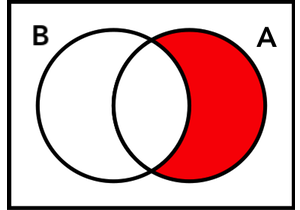
\includegraphics[width=0.3\textwidth]{images/set_difference.png}
    \end{center}
\end{definition}
\begin{definition}[Symmetric Difference]
    We define the \ul{symmetric difference}
    \[A\triangle B = (A\setminus B)\cup (B\setminus A).\]
    \begin{center}
        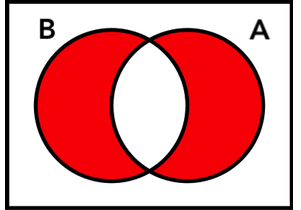
\includegraphics[width=0.3\textwidth]{images/set_sym_difference.png}
    \end{center}
\end{definition}
\begin{definition}[Set Product]
    We define the \ul{product} of $A$ and $B$ as
    \[A\times B = \{(a, b)\mid a\in A, b\in B\}\]
\end{definition}

\subsubsection{Relations}
\begin{definition}[Relations]
    A \ul{relation} $R$ between sets $A$ and $B$ is any subset of $A\times B$.

    If $(a, b)\in R$, we will think of $a$ ``being related'' to $b$.
\end{definition}

For now, consider $A = B$. We define a special set of relations.
\begin{definition}[Reflexive/Symmetric/Transitive Relations]\label{defn:rst-relations}
    We have the following definitions:
    \begin{enumerate}
        \item $R$ is \ul{reflexive} iff $(a, a)\in R, \forall a\in A$.\framedfootnote{$\forall$ is to say `for all'.}
        \item $R$ is \ul{symmetric} iff whenever $(a_1, a_2)\in R$, then $(a_2, a_1)\in R$.
        \item $R$ is \ul{transitive} iff whenever $(a_1, a_2)\in R$, and $(a_2, a_3)\in R$, then $(a_1, a_3)\in R$.
    \end{enumerate}
\end{definition}

\begin{definition}[Equivalence Relation]
    A relation $R$ that satisfies all conditions 1-3 in \cref{defn:rst-relations} is called an \ul{equivalence relation}.
\end{definition}

\begin{definition}[Equivalence Class]
    Given an element $a\in A$ with relation $R$, we write
    \[[a]_R \overset{\text{def}}{=} \{a' \in A\mid (a, a')\in R\}\]
    as the \ul{equivalence class} of $a$ (the set of all elements that are `related' to $a$).
\end{definition}
\begin{remark}
    Instead of writing $(a, a')\in R$, we write $a\sim_R a'$ or $a\sim a'$.
\end{remark}

\begin{proposition}[Distinct Equivalence Classes are Disjoint]
    If $R$ be an equivalence relation on $A$. Suppose $a_1, a_2\in A$. Then, either
    \[[a_1]_R = [a_2]_R\quad \text{or}\quad [a_1]_R\cap [a_2]_R = \emptyset\]
\end{proposition}
\begin{proof}
    We show that these statements cannot happen simultaneously, and that one or the other \emph{must} be true.

    The former is as follows: notice $a_1\in [a_1]_R$ because $a_1\sim a_1$ by $R$ reflexive. Since $[a_1]_R = [a_2]_R$, then $a_1\in [a_1]_R\cap [a_2]_R$. This implies that the intersection $[a_1]_R\cap [a_2]_R$ is nonempty, which is a contradiction.

    We now show that at least one has to happen. If $a_1\in [a_1]_R\cap [a_2]_R = \emptyset$, we are done. Otherwise, if $a_1\in [a_1]_R\cap [a_2]_R \neq \emptyset$, then $\exists\footnote{$\exists$ is to denote `there exists'.}a\in A$ such that $a\in[a_1]_R$ and $a\in[a_2]_R$.

    We claim \textsc{wlog} $[a]_R = [a_1]_R$. Suppose $a'\in [a]_R$, then $(a, a')\in R$. Since $(a,a')\in R$ and $(a_1, a)\in R$ (due to $a\in [a_1]_R$), transitivity gives $(a_1, a')\in R$ so $a'\in[a_1]_R$. Let's otherwise suppose $a'\in [a_1]_R$, so $(a_1, a')\in R$. Reflexivity gives $(a, a_1)\in R$ ($(a_1, a)\in R$ by $a\in [a_1]_R$), and by transitivity $(a,a_1)\in R$ and $(a_1, a')\in R$ gives $(a, a')\in R$ so $a'\in [a]_R$.\footnote{Wow, this is quite dense but the idea is to chain reflexivity and transitivity to get everything related to one another.}

    By symmetry, $[a]_R = [a_2]_R$, so $[a_1]_R = [a]_R = [a_2]_R$ which is as desired.
\end{proof}

Essentially, what we have shown, is that we can partition a set according to equivalence classes. All equivalence classes are either going to be the same or different. This is, equivalence relations form a \emph{partition} of a set. We can construct a set of partitions (disjoint subsets) of a set $S$. That is, ``equivalence classes partition $A$.''

\begin{definition}[Partition]
    A \ul{partition} of $A$ is a collection $\mathcal{P}$ of subsets of $A$ such that
    \begin{enumerate}
        \item $A = \bigcap_{S\in \mathcal{P}}S$,
        \item $S_i\cap S_j = \emptyset$ if $S_i\neq S_j$ for each $S_i, S_j\in \mathcal{P}$.
    \end{enumerate}
\end{definition}

With this definition, if $R$ is an equivalence relation, then $\mathcal{C}_R = \{[a]_R\mid a\in A\}$ is a partition of $A$.

We'll use all of this to define a function (which is the whole purpose of this course).

\subsubsection{Functions}
\begin{definition}[Function]
    Let $A, B$ be sets and $f$ be a relation between $A$ and $B$.

    We say $f$ is a \ul{function} from $A$ to $B$ and we write $f: A\to B$ iff the following holds:
    \begin{enumerate}
        \item $\forall a\in A$, there exists \emph{at least} one $b\in B$ s.t. $(a, b)\in f$. (all elements have an image)
        \item $\forall a\in A$, there exists \emph{at most} one $b\in B$ s.t. $(a, b)\in f$. (all elements have only one image)
    \end{enumerate}
    We write $f(a) = b$, and $b$ is the \ul{image} of $a$ by $f$. We call $A$ the domain of $f$, and $B$ the codomain of $f$\framedfootnote{I like to denote $B$ the codomain and the actual set of images the \emph{image} of $f$. And `range' is just ambiguous it seems.}.
\end{definition}
%!TEX root = ../notes.tex
\section{January 31, 2023}

\subsection{Properties of Functions}
\begin{definition}[Injectivity]
    A function $f: A\to B$ is \ul{injective} (one-to-one) if
    \[f(a_1) = f(a_2)\implies a_1 = a_2.\]
    ``No two elements in $A$ map to the same element in $B$.''
\end{definition}

\begin{definition}[Surjectivity]
    A function $f: A\to B$ is \ul{surjective} (onto) if
    \[\forall b\in B, \exists a\in A, \text{ s.t. }f(a) = b.\]
    ``Every element in $B$ has a preimage in $A$.''
    % \todo{Diagram}
\end{definition}

\begin{definition}[Functional Composition]
    Suppose $f: A\to B$ and $g: B\to C$ are functions, then $(g\circ f): A\to C$ with
    \[(g\circ f)(a) := g(f(a))\]
    % \todo{Diagram}
\end{definition}

\begin{proposition}
    Let $f: A\to B$, $g: B\to C$ be functions, then if $f, g$ are both injective, then so is $(g\circ f)$.

    The same holds if they are surjective.
\end{proposition}
\begin{proof}[Proof of injective part]
    Let $a, a'\in A$ be such that
    \begin{align*}
        (g\circ f)(a) & = (g\circ f)(a') \\
        g(f(a))       & = g(f(a'))       \\
        \intertext{With $g$ injective, therefore}
        f(a)          & = f(a')
        \intertext{With $f$ injective, we then have}
        a             & = a'
    \end{align*}
    Therefore, $(g\circ f)$ is injective.
\end{proof}

\begin{proof}[Proof of surjective part]
    We want to show that $\forall c\in C$, $\exists a\in A$ such that $g(f(a)) = (g\circ f)(a) = c$.

    Since $g$ is surjective, $\exists b\in B$ s.t. $g(b) = c$.

    Since $f$ is surjective, $\exists a\in A$ such that $f(a) = b$.

    Now, plugging in, $g(f(a)) = g(b) = c$. Therefore, exists such a pre-image $a\in A$ for every $c\in C$ under $(g\circ f)$. Hence, $(g\circ f)$ is surjective.
\end{proof}

\begin{definition}[Bijectivity]
    If $f: A\to B$ is injective and surjective, we call $f$ a \ul{bijection}.
\end{definition}

\begin{theorem}[Existence of Inverse]
    Let $f: A\to B$, then $\exists f^{-1}: B\to A$ such that
    \begin{align*}
        f^{-1}\circ f = \mathrm{id}_A \\
        f\circ f^{-1} = \mathrm{id}_B
    \end{align*}
    where
    \begin{align*}
        \Id_A: A\to A, \quad \forall a\in A, \Id_A(a) = a \\
        \Id_B: B\to B, \quad \forall b\in B, \Id_B(b) = b
    \end{align*}
    if and only if $f$ is a bijection.
\end{theorem}
\begin{proof}
    ~\begin{description}
        \item[$\Longleftarrow$:] Suppose $f: A\to B$ is a bijection. Then, we define $f^{-1}\subset B\times A$ as
            \[f^{-1} = \{(b, a)\mid (a, b)\in f\}\]
            It's clear that this is a relation. We check that $f^{-1}$ is a function.

            That is, we need to check that $\forall b\in B$, there exists one and only one $a\in A$ such that $(b, a)\in f^{-1}$.

            In other words, taking the definition of $f^{-1}$, we have to check that $\forall b\in B$, $\exists!\footnote{$\exists!$ as `exists exactly one'.} a\in A$ such that $(a, b)\in f$. This is exactly $f$ being bijective.

            Let's now show that
            \begin{align}
                f^{-1}\circ f & = \Id_A \label{eq:inverse-1} \\
                f\circ f^{-1} & = \Id_B \label{eq:inverse-2}
            \end{align}

            Let's first show \cref{eq:inverse-1}, suffices to show $f^{-1}(f(a))\overset{?}{=}a, \forall a$.

            $\forall a\in A$, $\exists b\in B$ such that $f(a) = b$, so $(a, b)\in f$. By definition, $(b, a)\in f^{-1}$ so $f^{-1}(b) = a$. Then $f^{-1}(f(a)) = f^{-1}(b) = a$.

            We do \cref{eq:inverse-2} very similarly.

        \item[$\Longrightarrow$:] Suppose $f: A\to B$ and $g\footnote{We use $g$ to reduce confusion with $f^{-1}$}: B\to A$ such that $g\circ f = \Id_A$ and $f\circ g= \Id_B$. We show that $f$ is a bijection.

            We first show injectivity. Suppose $f(a_1) = f(a_2)$, applying $g$ on both sides gives
            \begin{align*}
                g(f(a_1))  & = g(f(a_2))  \\
                \Id_A(a_1) & = \Id_A(a_2) \\
                a_1        & = a_2
            \end{align*}
            This gives us injectivity.

            We then show surjectivity. Let $b\in B$, we claim $\exists a\in A$ such that $f(a) = b$. Take $a := g(b)$, then $f(a) = f(g(b)) = b$. We've found such an $a$ such that $f(a) = b$, giving us surjectivity.
    \end{description}
    In both directions, this gives us the bijection.
\end{proof}

\begin{remark}
    Let $f: A\to B$ be a bijection, with $A$ and $B$ finite. We have that $A$ has $n$ elements $\iff$ $B$ has $n$ elements. That is, $A$ and $B$ have equal cardinality.

    This extends to arguments on infinite sets too, like between $\ZZ$ and $\QQ$. $\QQ$ and $\RR$ or $\ZZ$ and $\RR$ have different cardinalities and hence don't have bijections.
\end{remark}

If $f: A\to B$ is not a bijection, we cannot define an inverse in the same way as we did before. But, we can consider the inverse image.

\begin{definition}[Inverse Image]
    Given function $f: A\to B$, $C\subseteq B$ we define the \ul{inverse image} of $C$ as
    \[f^{-1}(C) := \left\{ a\in A\mid f(a)\in C \right\}\]
    ``The set of $a\in A$ that take me somewhere in $C$.''
\end{definition}

If $C = \{b\}$, we get all elements mapped to $b$. That is,
\[f^{-1}(\{b\}) = \left\{ a\in A\mid f(a) = b \right\}\]

\subsection{Cardinality}

%!TEX root = ../notes.tex
\section{February 2, 2023}
\subsection{Natural Numbers, \emph{continued}}
\recall we defined the natural numbers $\NN$. We had a \emph{successor} function $s$ where $2 = s(1)$, $3 = s(2)$, and so on\dots

\begin{definition}
    We define
    \begin{enumerate}[a.]
        \item For any $n\in \NN$, $n+1 := s(n)$.
        \item For every $m, n\in\NN$ $n + s(m) := s(n + m)$.
    \end{enumerate}
\end{definition}

\begin{proposition}
    We can check that
    \begin{enumerate}
        \item $\forall m, n\in \NN$, $m+n = n+m$.
        \item $\forall n, m, r\in\NN$,
              \[m + (n + r) = (m + n) + r\]
        \item $\forall n, m\in \NN$, $n + m\neq N$.\framedfootnote{We note that $0\not\in\NN$.}
        \item $s$ is a bijection from $\NN$ to $\NN\setminus\{1\}$.
    \end{enumerate}
\end{proposition}
\begin{proof}[Proof of 4]
    We note that by the Peano axioms, $s$ doesn't map any element to $1$. Then, $s: \NN\to\NN\setminus\{1\}$.

    We show that $s$ is bijective. Consider
    \[S = \{1\}\cup \left\{ s(n)\mid n\in\NN \right\}.\]
    Suffices to show that $S = \NN$. We know that $1\in S$ by construction, and if $n\in S$, $n\in \NN$, $s(n)\in S$ by construction, then by axiom (3), $S = \NN$.

    Hence if $k\neq 1$, $\exists n$ such that $k = s(n)$. Since $s$ is injective by axiom (2), $s$ is bijective.
\end{proof}

Now that we have a bijection, we can define predecessors:

\begin{definition}[Predecessor]
    We can define $n-1$ for $n\neq 1$ by saying that $n-1$ is the element such that
    \[(n-1) + 1 = n.\]
\end{definition}

\begin{definition}[Ordering]
    We say that $m\leq n$ for $m, n\in\NN$ if either $m = n$ or $m + a = n$ for some $a\in \NN$.

    Moreover, ``$\leq$'' is a partial order that satisfies $\forall m, n \in\NN$, $m\leq n$ or $n\leq m$ (which makes $\leq$ a total order).
\end{definition}

\begin{definition}[Partial Order]
    A partial order $R$ is a relation such that
    \begin{enumerate}
        \item $a R a$,
        \item $a R b, b R a \Rightarrow a = b$,
        \item $a R b, b R c \Rightarrow a R c$.
    \end{enumerate}
\end{definition}

\begin{definition}[Multiplication]
    We define multiplication by
    \begin{align*}
        \forall n\in\NN, \qquad n\cdot 1 & = n             \\
        n\cdot s(m)                      & = n + n\cdot m.
    \end{align*}
\end{definition}

\begin{proposition}
    Our definition of multiplication satisfies the following: $\forall n, m, r, s\in\NN$,
    \begin{enumerate}
        \item \emph{(Distributivity)} $n\cdot(m + r) = n\cdot m + n\cdot r$
        \item \emph{(Commutativity)} $n\cdot m = m\cdot n$
        \item \emph{(Associativity)} $(n\cdot m)\cdot r = n\cdot (m\cdot r)$
        \item If $n < m$ and $r \leq s$, then $r\cdot n < s\cdot m$.
    \end{enumerate}
\end{proposition}

\subsection{Cardinality \& Natural Numbers}
For each $n\in\NN$, consider
\[J_n = \left\{ m\in\NN\mid m\leq n \right\}.\]
That is, $J_1 = \{1\}$, $J_2 = \{1, 2\}$.
\begin{proposition}
    For $n\geq 1$,
    \[J_{n+1} = J_n\cup \left\{ n+1 \right\}.\]
\end{proposition}
\begin{proof}
    We prove by showing subset inclusion in both directions:
    \begin{description}
        \item[$\supset$:] Let $k\in J_n\cup \{n+1\}$. If $k = n+1$, $k\in J_{n+1}$. If $k\in J_n$, then $k\leq n$ and since $n\leq n+1\Rightarrow k\leq n+1\Rightarrow k\in J_{n+1}$.
        \item[$\subset$:] Let $k\in J_{n+1}$. If $k\in J_n$, we are done. If $k\not\in J_n$, then $k \not\leq n \Rightarrow k \geq n+1$. But $k\in J_{n+1}\Rightarrow k\leq n+1$. So necessarily, $k = n+1$.
    \end{description}
    Which is as desired.
\end{proof}

\begin{definition}[Cardinality, \emph{again}]
    We say that a set $A$ has \ul{cardinality}\framedfootnote{This is unfortunately an abuse of notation.} $n$ if
    \[A\simeq\framedfootnote{We use $\sim$ to denote a relation, and $\simeq$ to denote a bijection.} J_n\framedfootnote{This is in a model that assumes $0\in\NN$, unfortunately, which is a bit confusing.}.\]
    In this case, we say $A$ is finite and write $\#(A) = n$.

    If $A$ is not related to any $J_n$, we say that $A$ is \ul{infinite}.
\end{definition}

\begin{lemma}
    Let $A, B$ be finite\framedfootnote{They don't need to be finite, but then the comparison of cardinalities is a bit wishy-washy.} sets. If $A\subset B$, then $\#(A)\leq \#(B)$.
\end{lemma}
\begin{proof}
    Define $f : A\to B$ with $a\mapsto a$. $f$ is injective by definition.

    This is a bijection with a subset of $B$, therefore the cardinality has to satisfy $\#(A)\leq \#(B)$.
\end{proof}

\begin{theorem}\label{thm:NN-countable-infinity}
    $\forall n\in \NN$,
    \[\#(J_n) < \#(J_{n+1}) < \#(\NN)\]
\end{theorem}
\begin{proof}
    If we replace the first $<$ by $\leq$, then this is easy by the previous lemma.

    We assume we already know\footnote{Note from me: why can't we claim $\#(J_n) = n$ by definition of cardinality?}
    \begin{equation}\label{eqn:cardinalities-theorem-assumption}
        \#(J_n)\neq \#(J_{n+1}), \forall n,
    \end{equation}
    we want to show that $\#(J_n)\neq \#(\NN), \forall n$.

    Assume there exists some $n$ such that
    \[\#(\NN) = \#(J_n)\]
    Then we have
    \[\#(J_{n+1})\leq \#(\NN) = \#(J_n)\]
    which is a contradiction.
\end{proof}

\begin{proof}[Proof of \cref{eqn:cardinalities-theorem-assumption}]
    We induct on $n$.
    \begin{description}
        \item[Base case $n = 1$.] $J_1 = \{1\}$ and $J_2 = \{1, 2\}$. Then $\#(J_1) < \#(J_2)$, since we can't define a bijection.
        \item[Inductive step.] Suppose that $\#(J_n)\neq \#(J_{n+1})$. We wish to prove $\#(J_{n+1}) \neq \#(J_{n+2})$. By contraposition, assume there exists a bijection $f: J_{n+1}\to J_{n+2}$. Then, $\exists k\in J_{n+1}$ such that $f(k) = n + 2$. Define $h: J_{n+1}\to J_{n+1}$ by
            \[h(m) := \begin{cases}
                    m   & \text{if }m\not\in \{k, n+1\} \\
                    m+1 & \text{if }m=k                 \\
                    k   & \text{if }m = n+1
                \end{cases}\]
            Let $\hat f = f\circ h : J_{n+1} \to J_{n+2}$, a bijection. $\hat f$ maps $n+1\mapsto n+2$. Defining $g(x) = \hat f(x)$ for $x\in J_n$ ($\hat f$ restricted to $J_n$ so $g : J_n\to J_{n+1}$) completes the contraposition.
    \end{description}
    Which gives the general statement of \cref{eqn:cardinalities-theorem-assumption}.
\end{proof}

\begin{corollary}
    If $A\simeq \NN$, $A$ is infinite.

    We say in this case that $A$ is \ul{countable}.

    If $A$ is infinite and $\#(A)\neq \#(\NN)$\framedfootnote{That is, $A\not\simeq \NN$.}, then we say that $A$ is \ul{uncountable}.
\end{corollary}
\begin{proof}
    If $A$ were finite, then $A\simeq J_n$ for some $n$ which is impossible by \cref{thm:NN-countable-infinity}.
\end{proof}
\begin{example}
    $\NN$ is countable, $\QQ$ is countable, $\RR$ is uncountable.
\end{example}

\begin{corollary}
    Let $S$ be an infinite subset of $\NN$. Then $S$ is countably infinite.
\end{corollary}

\begin{definition}[Countability]
    We say that $A$ is \ul{countable} if $A$ is finite or countable infinite.
\end{definition}
%!TEX root = ../notes.tex
\section{February 7, 2023}
\subsection{Natural Numbers, \emph{continued}}
\begin{theorem}
    Let $S$ be an infinite subset of $\NN$. Then $S$ is countably infinite.
\end{theorem}
\begin{proof}
    The objective is to construct a bijection between $S$ and $\NN$. We will do this inductively.

    Let $f(1)$ be the smallest element\footnote{Within resonable context, we assume that $\NN$ is well-ordered. That is, every subset has a least element.} of $S$ for $f : \NN\to S$.

    Assuming we have defined $f(1), f(2), \dots, f(n)$, we define $f(n+1)$ to be the smallest element of $S \setminus \{f(1), f(2), \dots, f(n)\}$.

    By construction, $f$ is bijective.
\end{proof}

Recall \cref{defn:countability}:
\begin{definition*}[Countability]
    We say that $A$ is \ul{countable} if it is finite or countably infinite.
\end{definition*}

\begin{theorem}
    Let $\mathcal{C}$ be a countable collection\framedfootnote{A `collection' usually refers to a collection of sets.} of countable sets.

    Then the union $\displaystyle \bigcup_{A\in \mathcal{C}}A$ is countable.
\end{theorem}

We can do something like this:
\begin{center}
    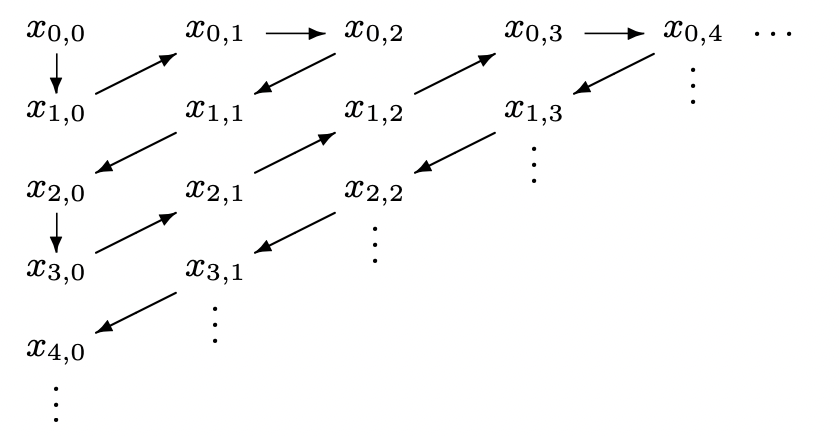
\includegraphics[width=0.5\textwidth]{images/countable_collection_of_sets.png}
\end{center}

\begin{proof}
    Again, we try to construct a bijection $f$ from $\NN$. We list all the elements of $\bigcup_{A\in\cC}A$ in a sequence. This will give $f(1), f(2), \dots$ and so on.

    Since each $A$ is countable, we may list its elements. The collection $\cC$ is also countable. We can arrange every row to be an element of $\cC$.


    \[\begin{array}{c|cccc}
            A_1    & a_1    & a_2    & a_3    & \cdots \\
            A_2    & b_1    & b_2    & b_3    & \cdots \\
            A_3    & c_1    & c_2    & \cdots          \\
            A_4    & d_1    & \cdots                   \\
            \vdots & \vdots & \ddots
        \end{array}\]

    We then count the elements using diagonals (or a zig-zag), and remove duplicates\footnote{This is a bit wishy-washy, but we're only removing elements here so we remain in the `countable' territory.}.
\end{proof}

\subsection{Before We Get to the Real Numbers}
Let's begin by proving the following theorem.
\begin{theorem}
    $\sqrt{2}$ is not rational.
\end{theorem}
\begin{proof}
    Assume not, that we can write $\sqrt{2} = \frac{m}{n}$, for $m, n\in\ZZ$, $N\neq 0$ and $m, n$ coprime.

    Then, $2n^2 = m^2$. So, $m$ is even. Writing $m = 2m'$, $2n^2 = 4m'^2$, which in particular implies $n$ is even, which is a contradiction.

    It had better be, then, that $\sqrt{2}$ is irrational.
\end{proof}

We now show more, namely that we can get arbitrarily close to irrational numbers by rational numbers\footnote{This is to say, $\QQ$ is \emph{dense} in $\RR$.}.
\begin{theorem}
    If $q\in\QQ$ satisfies $0 < q^2 < 2$, then we can find $\bar{q}\in\QQ$ such that $q^2 < \bar{q}^2 < 2$. Similarly if $r\in\QQ$ satisfies $2 < r^2$, then we can find $\bar{r}\in\QQ$ such that $2 < \bar{r}^2 < r^2$.
\end{theorem}
\begin{proof}
    We'll just prove the first part; the second part is similar.

    Suppose $q > 0$, define
    \[\bar{q} = q + \frac{2 - q^2}{2 + q}.\]
    then $\bar{q} > q$ and
    \begin{align*}
        \bar{q}^2 - 2 & = q^2 + \left( \frac{2-q^2}{q+2} \right)^2 + \frac{2q(2-q^2)}{2+q} - 2                                       \\
                      & = \frac{(q^2 - 2)(q+2)^2 + (2-q^2)^2 + (2-q^2)2q(2+q)}{(q+2)^2}                                              \\
                      & = \frac{q^2 - 2}{(q+2)^2}\left[ \cancel{q^2} + 4 + \cancel{4q} + \cancel{q^2} - 2 - \cancel{2q(2+q)} \right] \\
                      & = \frac{2(q^2 - 2)}{(q+2)^2}
    \end{align*}
    which is surely negative.
\end{proof}
\begin{corollary}
    The set
    \[\left\{ q\in\QQ\mid q^2 < 2 \right\}\]
    \textbf{does not} have a largest element.
\end{corollary}

\begin{definition}[Upper Bound]
    If $A$ is a set with a partial ordering $\leq$, we say that $a\in A$ is an \ul{upper bound} for a subset $B\subset A$ if $b\leq a$ $\forall b\in B$.

    We say that $a$ is a \ul{least upper bound} for $B$ if whenever $a'$ is an upper bound for $B$, then $a\leq a'$.
\end{definition}

\begin{lemma}
    If $a$ is a least upper bound for $B$, then $a$ is unique.
\end{lemma}
\begin{proof}
    Assume $a, a'$ are both least upper bounds for $B$. By definition, both $a, a'$ are upper bounds. \textsc{wlog}, if $a$ is a least upper bound and $a'$ an upper bound, $a\leq a'$. Similarly, $a'\leq a$. Hence, $a = a'$.
\end{proof}
Now that we have proved uniqueness, we can give $a$ a name:
\begin{definition}[Supremum \& Infimum]
    We define $\sup B := a$ when $a$ is the least upper bound of $B$.

    Similarly, $\inf B := a$ when $a$ is the greatest lower bound of $B$.
\end{definition}
\begin{definition}[Least-Upper-Bound Property]
    Let $A$ be a totally ordered set with order $\leq$. We say that $A$ has the least upper bound property if each nonempty subset of $B\subset A$ with an upper bound in $A$ has a least upper bound in $A$.
\end{definition}

% \intentionalpagebreak
\subsection{The Real Numbers}

\begin{definition}
    A \ul{field} $F$ is a set with two operations: $+, \cdot$.

    The $+$ operation satisfies:
    \begin{description}
        \item[Closure.] $x, y\in F\Rightarrow x + y\in F$.
        \item[Commutativity.] $x + y = y + x$, $\forall x, y\in F$.
        \item[Associatifity.] $(x + y) + z = x + (y + z)$, $\forall x, y, z\in F$.
        \item[Identity.] $\exists 0$ such that $0 + x = x$ $\forall x\in F$.
        \item[Inverses.] $\forall x\in F$, $\exists -x\in F$ such that $x + (-x) = 0$.
    \end{description}

    And a $\cdot$ operation that satisfies:
    \begin{description}
        \item[Closure.] $x, y\in F\Rightarrow x \cdot y\in F$.
        \item[Commutativity.] $x \cdot y = y \cdot x$, $\forall x, y\in F$.
        \item[Associatifity.] $(x \cdot y) \cdot z = x \cdot (y \cdot z)$, $\forall x, y, z\in F$.
        \item[Identity.] $\exists 1 \neq 0$ such that $1\cdot x = x$, $\forall x\in F$.
        \item[Inverse.] $\forall x\neq 0$, $\exists x^{-1}\in F$ such that $x\cdot x^{-1} = 1$
    \end{description}

    Together, we also have
    \begin{description}
        \item[Distribution.] $\forall x, y, z\in F$, $x\cdot (y + z) = x\cdot y + x\cdot z$.
    \end{description}

    In other words, a field $F$ is a commutative ring with multiplicative inverse.
\end{definition}
\begin{definition}
    An \ul{ordered field} is a field $F$ which is an ordered set such that
    \begin{enumerate}
        \item $x + y < x + z$ if $x, y, z\in F$ and $y < z$.
        \item $x\cdot y > 0$ if $x, y\in F$ and $x > 0$, $y > 0$.
    \end{enumerate}
\end{definition}
\begin{example}
    $\QQ, \RR$ are ordered fields. $\NN, \ZZ$ are not fields.
\end{example}

\begin{theorem}[Archimedian Property]
    \label{thm:archimedian-property}
    Given $x, y\in \RR$, $x > 0$. Then $\exists n\in \ZZ$ such that $nx > y$.
\end{theorem}
\begin{proof}
    We argue by contradiction. Assume such $n$ doesn't exists.

    Then take set
    \[A = \left\{ nc \mid n\in\NN \right\}\]
    which is bounded by $y$.

    Therefore, if it has supremum\footnote{$\RR$ has the least upper bound property.} $s$, $s-x < s$, so $s-x$ is not an upper bound of $A$ (otherwise $s$ is not a supremum). Then, $\exists a\in A$ (otherwise $s-x$ would have been an upper bound) such that $a \geq s - x$, which means $\exists m\in \NN$ such that $mx > s-x$. This implies that $s < (m+1)x$ but $m+1\in A$, which is a contradiction.
\end{proof}

\begin{corollary}
    Let $x, y\in\RR$ with $x < y$. Then $\exists q\in \QQ$ such that $x < q < y$. This is to say, ``in between any two real numbers lies rational numbers.''
\end{corollary}
\begin{proof}
    By \cref{thm:archimedian-property} applied to $y-x$ and $1$. Then $\exists n\in\ZZ$ such that
    \[n(y-x) > 1\]
    and we can also find $m_1, m_2\in\NN$ such that
    \[m_1 > nx, m_2 > -nx\]
    by the Archimedian property again.
    which implies
    \[-m_2 < nx < m_1\]
    Then, $\exists m\in \NN$ such that $m-1 \leq nx < m$\footnote{By contradiction, if there is no such $m$ we incur the previous statement}. Which implies that
    \[nx < m \leq 1 + nx < ny\]
    which then gives
    \[x < \frac{m}{n} < y\]
    which is as desired. $\frac{m}{n}$ is precisely a rational between real $x$ and $y$.
\end{proof}

\begin{theorem}
    For every $x\in\RR$ with $x > 0$, $n > 0\in \NN$, $\exists! y > 0$ such that $y^n = x$.
\end{theorem}
\begin{proof}
    We prove uniqueness. Suppose by contradiction that \textsc{wlog} $y_1 < y_2$ such that $y_1 ^ n = x$ and $y_2^n = x$. Contradiction by $y_1^n < y_2^n$.

    We now start the proof for existence. Let
    \[E = \{t\mid t^n < x\}\]
    If $t = \frac{x}{x+1}$, then $t < x$ and $0 < t < 1$. So $t^n < t < x$ so $E$ is not empty.

    If $t > 1 + x$, $t^n \geq t > x$. We've found an upper bound of $E$. Then, $\exists y = \sup E$.

    We'll leave it here that $E$ has a supremum, and continue next time.
\end{proof}
%!TEX root = ../notes.tex
\section{February 9, 2023}
\subsection{Real Numbers, \emph{continued}}
\recall from last time that we were trying to prove
\begin{theorem*}
    $\forall x\in \RR, x > 0$ and $\forall n\in \NN, n > 0$,
    \[\exists! y > 0 \text{ s.t. }y^n = x.\]
\end{theorem*}
\begin{proof}
    Define $E$ as
    \[E := \left\{ t\mid t^n < x \right\}.\]
    $E$ has an upper bound $x$ and by the least upper bound property, $\exists y = \sup(E)$.

    Our objective is to show that $y^n = x$. We use the identity that
    \begin{align*}
        b^n - a^n & = (b-a)(b^{n-1} + ab^{n-2} + a^2b^{n-3} + \cdots + a^{n-1}).
        \intertext{Assuming that $a, b$ positive, and bounding $b^{n-1} + ab^{n-2} + \cdots < nb^{n-1}$,}
        b^n - a^n & < (b-a)nb^{n-1}
    \end{align*}
    if $0 < a < b$.

    For the sake of contradiction, first assume $y^n < x$. Choose $0 < h < 1$ such that
    \[h < \frac{x - y^n}{n(y+1)^{n-1}}.\]
    Then, $(y+1)^n - y^n < hn(y+h)^{n-1}$, this is also bounded by $<hn(y+1)^{n-1} = x-y^n$ so we have that $(y+h)^n < x$.

    Then $y+h\in E$. But we defined $y$ to be the supremum of $E$, which is a contradiction.

    We complete our `squeeze' with assuming (again, for the sake of contradiction) that $y^n > x$. We choose
    \[h = \frac{y^n - x}{ny^{n-1}} > 0.\]
    Since $y^n - x < ny^n$, $h < y$. Then we can show that
    \[y^n - (y-h)^n < hny^{n-1} = y^n - x\]
    so $(y-h)^n > x$. This again, contradicts $y$ being a least upper bound since $y-h < y$ and $y-h$ is an upper bound.

    Hence the least upper bound of $E$ is the $n$-th root of $x$ exactly by our two contradictions.
\end{proof}

\subsection{Metric Spaces}
\emph{We'll do some topology for the next few classes or so.}
\begin{definition}[Metric Space]
    A set $X$ and a function $d : X\times X \to \RR$ is a \ul{metric space} if we have the following properties:
    \begin{description}
        \item[Nonnegative.] $d(x, y) \geq 0$, furthermore $d(x, y) = 0\iff x = y$.
        \item[Symmetric.] $d(x, y) = d(y, x)$.
        \item[Triangle Inequality.] $d(x, y) \leq d(x, z) + d(z, y)$.
    \end{description}
    We will call $d$ a \ul{distance}.
\end{definition}
\begin{example}
    $X = \RR^n$ with $d(\vec{a}, \vec{b}) = |\vec{a} - \vec{b}|$ is a metric space.
\end{example}
\begin{example}\label{ex:trivial-metric-space}
    $X$ arbitrary, and
    \[d(x, y) = \begin{cases}
            1 & \text{ if }x\neq y \\
            0 & \text{ if }x = y
        \end{cases}\]
    is also a metric space.
\end{example}
\begin{example}
    $X = \left\{ f\mid f \text{ bounded and }f : [0, 1]\to\RR\right\}$ with
    \[d(f, g) = \sup_{x\in[0, 1]}\left\{ |f(x) - g(x)| \right\}\]
    is a metric space.
\end{example}

\subsubsection{Open and Closed Sets}
The mental image for these are open and closed intervals on the real number line.
\begin{definition}[Neighborhood]
    Let $r > 0$. The \ul{neighborhood} of radius centered at $x \in X$ is
    \[B_r(x) = \left\{ y \in X \mid d(x, y) < r \right\}.\]
\end{definition}
\begin{example}
    In $\RR$, with $d = |x - y|$, we get the open interval
    \[B_r(x) = \left\{ y\mid x - r < y < x + r \right\}\]
\end{example}
\begin{example}
    In $\RR^n$ with $d(\vec{x}, \vec{y}) = |\vec{x} - \vec{y}|$, we get the open ball
    \[B_r(\vec{x}) = \left\{ \vec{y} = (y_1, \dots, y_n)\mid (x_1 - y_1)^2 + \cdots + (x_n - y_n)^2 < r^2 \right\}.\]
\end{example}
\begin{example}
    In \cref{ex:trivial-metric-space}, a neighborhood with radius $0.5$ is the point itself, and a neighborhood with radius $2$ is the entire space.
\end{example}

Let $(X, d)$ be a metric space.
\begin{definition}[Open Set]
    A set $Y\subset X$ is \ul{open} if $\forall y\in Y$, $\exists r > 0$\framedfootnote{This $r$ may depend on our $y$.} such that $B_r(y)\subset Y$.
\end{definition}

\begin{proposition}
    Any neighborhood is open.
\end{proposition}
\begin{proof}
    Let $x\in X$, $r > 0$. We look at $B_r(x)$.

    $\forall y\in B_r(x)$, we want to find $s$ such that
    \[B_s(y) \subset B_r(x)\]
    Let $s = r - d(x, y)$. Let $z\in B_s(y)$. We wish to show that $z\in B_r(x)$, that is, $d(z, x) < r$.

    Invoking the triangle inequality,
    \[d(z, x) \leq d(z, y) + d(y, x) < s + d(x, y) = r - d(x, y) + d(x, y).\]
    This gives that every point in $B_s(y)$ is in $B_r(x)$, so $B_s(y)\subset B_r(x)$. Hence, every neighborhood is open.
\end{proof}
\begin{example}
    In $\RR$, the only intervals which are open are open intervals\framedfootnote{This looks...tautological.}.
\end{example}
\begin{example}
    In $\RR^2$, the set
    \[\{(x, y)\mid y > 0\}\cup \{(x, y)\mid y < -1\}\]
    is open.
\end{example}
\begin{remark}
    Not being open \textbf{does not} imply a set is closed.
\end{remark}
\begin{proposition}
    Let $\cC$ be a collection of open sets.
    \begin{enumerate}[(1)]
        \item $\displaystyle \bigcup_{O\in \cC} O$ is open.
        \item $\displaystyle \bigcap_{O\in \cC} O$ is open if $\cC$ is finite.
    \end{enumerate}
    If $\cC$ is infinite, (2) might fail.
\end{proposition}
\begin{example}
    For example,
    \[O_n = \left( 1 - \frac{1}{n}, 1 + \frac{1}{n} \right)\]
    Then
    \[\bigcap O_n = \{1\}\]
\end{example}
\begin{proof}[Proof of (1).]
    Let $x\in \bigcup_{O\in \cC} O$. Then there exists $O\in \cC$ such that $x\in O$, which we denote $O_x$.

    Then, $\exists r$ such that $B_r(x)\subset O_x \subset \bigcup_{O\in \cC} O$. Hence, $\bigcup_{O\in \cC} O$ is open.
\end{proof}
\begin{proof}[Proof of (2).]
    Let $\cC = \{O_1, O_2, \dots, O_n\}$. Let $x \in \bigcap_{O\in \cC} O$. Then $x\in O_i$ for all $i$. Since each $O_i$ is open, there exists $r_i$ such that $B_{r_i}(x)\subset O_i$.

    Let $r = \min_i r_i$. Since the $\cC$ is finite, the minimum is strictly positive. Then $B_r(x)\subset B_{r_i}(x), \forall i$, so $B_r(x)\subset O_i, \forall i$. Therefore, $B_r(x)\in \bigcap_{O\in \cC} O$.
\end{proof}

\begin{definition}[Interior Point]
    An \ul{interior point} of $Y\subset X$ is a point $y\in Y$ such that $\exists r > 0$ such that $B_r(y)\subset Y$.

    We define
    \[\mathring Y  := \text{the set of interior points of }Y\]

    $Y\text{ open}\iff Y = \mathring Y$.
\end{definition}
\begin{example}
    $\mathring {[0, 1]} = (0, 1)$.

    $\mathring \QQ = \emptyset$.
\end{example}

\begin{definition}[Closed Set]
    A set $Y$ is \ul{closed} if $X\setminus Y$\framedfootnote{Sometimes, $Y^c$ is used to denote $X\setminus Y$, the complement of $Y$ in $X$.} is open.
\end{definition}
\begin{remark}
    A set can be open \emph{and} closed, or neither.

    For example, $\empty$ and $X$ are both open and closed.
\end{remark}

\begin{proposition}
    Let $\cC$ be a collection of closed sets. Then
    \begin{enumerate}[(1)]
        \item $\displaystyle \bigcap_{C\in \cC} C$ is closed.
        \item $\displaystyle \bigcup_{C\in \cC} C$ is closed if $\cC$ is finite.
    \end{enumerate}
\end{proposition}
\begin{proof}
    Let $C = X - O$ for some open set $O$.
    \[\bigcup_{c\in\cC}(X - O) = X = \bigcap_{O\in \cC}O\]
    Combined with the equivalent proposition for open sets completes this proof.
\end{proof}

\subsubsection{Limit Points}
\begin{definition}[Limit Point]
    Let $Y\subset X$. A point $x\in X$ is a \ul{limit point} of $Y$ if $\forall r > 0$, $\exists y\in Y$ such that $y\neq x$ and $y \in B_r(x)$. We denote
    \[Y' = \{y\mid y\text{ is a limit points of Y}\}.\]
\end{definition}
%!TEX root = ../notes.tex
\section{February 14, 2023}
The first quiz will definitely be after we get homework 2 back. Definitions on the quiz will come from lecture and the reading. Midterm will be around Spring break.

\subsection{Metric Spaces, \emph{continued}}
\subsubsection{Limit Points}
Recall that we left off at limit points last lecture.
\begin{example}
    The following are examples of sets and limit points:
    \begin{enumerate}
        \item $0$ is a limit point of the set
              \[\left\{ 0, \frac{1}{2}, \frac{1}{3}, \frac{1}{4}, \dots \right\}.\]
        \item $\{1, 2, 3\}\subset \RR$ has no limit points.
        \item In $\RR^2$,
              \begin{align*}
                  S  & = B_1(0)\cup \left\{ (x, 0)\mid x\in\RR \right\}\cup \{(10, 10)\}
                  \intertext{has limit points}
                  S' & = \underbrace{\{(x, y)\mid x^2 + y^2 \leq 1\}}_{\text{closed ball}}\cup \left\{ (x, 0)\mid x\in\RR \right\}.
              \end{align*}
              We note that nothing can approach $(10, 10)$ thus this is not a limit point. The open ball gives rise to the closed ball, and we also have the axis as well.
    \end{enumerate}
\end{example}

\begin{proposition}
    $x\in X$ is a limit point of $Y$ iff $\forall r>0$, $\exists$ infinitely many points of $Y$ in $B_r(x)$.
\end{proposition}
\begin{proof}
    ~\begin{description}
        \item[$\Longleftarrow$:] This falls from the definition. In fact, this is a stronger statement than the definition.

            Since $\forall r > 0$ there exists infinitely many points in $B_r(x)$, then there exists $y\neq x$ in $B_r(x)$.
        \item[$\Longrightarrow$:] Suppose otherwise, that there exists some $r > 0$ such that there doesn't exist infinitely many points of $Y$ in $B_r(x)$ (say there are finitely many points of $Y$ in $B_r(x)$). Let us call these points $y_1, \dots, y_n$. Let $r_0 = \min_{y_i\neq x}\{d(y_i, x)\} > 0$ (we're done if this set is empty).

            Then $B_{r_0}(x)\cap Y = \{x\}$, and $x$ is not a limit point of $y$, which is a contradiction.
    \end{description}
    Which concludes the bidirectional.
\end{proof}

\subsubsection{Closedness}

\begin{theorem}\label{thm:limit-points-in-closed}
    $Y$ is closed if and only if $Y' \subset Y$.
\end{theorem}
\begin{proof}
    ~\begin{description}
        \item[$\Longrightarrow$:] Suppose $Y$ is closed. Let $y \in Y'$, we wish to show that $y\in Y$. We argue by contradiction, suppose $y\not\in Y$, then $y\in X\setminus Y$ which is open. So, $\exists r > 0$ such that $B_r(y)\subset X\setminus Y$. Then, $B_r(y)\cap Y = \emptyset$ (since it is in $X\setminus Y$). This is a contradiction with $y\in Y'$.
        \item[$\Longleftarrow$:] Suppose $Y'\subset Y$. We want to show that $X \setminus Y$ is open.

            Let $z\in X\setminus Y$. Since $z\not\in Y$, $z\not\in Y'$ since $Y'\subset Y$. Then, $\exists r > 0$ such that $B_r(z)\cap Y$ has no points $p\neq z$ such that $p\in Y$. Then $B_r(z)\subset X\setminus Y$ implies $X\setminus Y$ is open.
    \end{description}
    Which is as desired.
\end{proof}

\begin{definition}[Closure]
    The \ul{closure} of $Y$ is $\overline{Y} = Y\cup Y'$.
\end{definition}

\begin{theorem}
    Let $\cC$ be a collection of sets $C\subset X$ such that $C$ is closed and $Y\subset C$. Then
    \[\overline{Y} = \bigcap_{C\in\cC}C.\]
    That is, $\overline{Y}$ is the smallest closed superset of $Y$.
\end{theorem}
\begin{proof}
    ~\begin{description}
        \item[Case $\subset$:] Let $y\in Y$ or $y\in Y'$, we want to show that $y\in \bigcap_{C\in\cC}C$. That is to say, it is in every superset of $Y$.

            If $y\in Y$, then $y\in Y\subset C$ by the definition of $C$.

            If $y\in Y'$, we pick arbitrary $C$. Since $y$ is a limit point of $Y$, $y$ is also a limit point of $C$. Since $C$ is closed, $y\in C$ by \cref{thm:limit-points-in-closed}. Since our choice of $C$ was arbitrary, it holds true for all $C$.

        \item[Case $\supset$:] We will show that $\overline{Y}\in \cC$. Since $\overline{Y}\supset Y$, we only need to show that $\overline{Y}$ is closed.

            If $x\not\in \overline{Y}$, then $x\not\in Y$ and $x\not\in Y'$. So $\exists r > 0$ such that $B_r(x)\cap Y = \emptyset$.

            Since $B_r(x)$ is open, each point has a neighborhood centered in $B_r(x)$, this means that the neighborhood doesn't intersect $Y$\footnote{Assume otherwise, then $z\in B_r(x)$ and $z\in Y'$, but we can squeeze a ball $B_{r'}(z)\subset B_r(x)$ which is disjoint from $Y'$.}. For each point in $B_r(x)$, that point is \emph{neither} in $Y$ nor a limit point of $Y$.

            Then, $B_r(x)\subset X\setminus \overline{Y}$, so $X\setminus \overline{Y}$ is open, then $\overline{Y}$ is closed.
    \end{description}
    Which is as desired.
\end{proof}

\begin{corollary}
    $Y = \overline{Y}$ if and only if $Y$ is closed.
\end{corollary}
\begin{proof}
    ~\begin{description}
        \item[$\Longrightarrow$:] Falls from the proof just now.
        \item[$\Longleftarrow$:] $Y$ is closed so $Y'\subset Y$ so $\overline{Y} = Y\cup Y' = Y$.
    \end{description}
    as desired.
\end{proof}

\subsubsection{Compactness}
\begin{definition}[Compactness]
    A subset $K$ of a metric space $(X, d)$ is \ul{compact} if for every collection $\cC$ of open sets such that $K\subset \bigcup_{C\in \cC}C$, one can extract a finite collection $C_1, C_2, \dots, C_n$ such that $K\subset \bigcup_{i=1}^n C_i$.

    $\cC$ is referred to as an \ul{open cover} of $K$, and $C_1, \dots, C_n$ is referred to as a \ul{finite subcover} of $K$.
\end{definition}

\begin{definition}[Boundedness]
    A set $E\subset X$ is \ul{bounded} if $\exists x\in X, R > 0$ such that $E\subset B_R(x)$.
\end{definition}
\begin{theorem}
    Any compact set $K\subset X$ is bounded.
\end{theorem}
\begin{proof}
    Fix arbitrary $x$. Take collection $\cC = \left\{ B_R(x) \mid R = 1, 2, \dots \right\}$.

    We show first that $\cC$ is an open cover. $\cC$ being open is clear, since each set is open. We show it is a cover. For any $y\in K$, $y\in B_R(x)$ for every $R > d(x, y)$. So $\cC$ is an open cover.

    Since $\cC$ is compact, then there exists a finite subcover $B_{R_1}(x), B_{R_2}(x), \dots, B_{R_n}(x)$. Take $R = \max\{R_1, \dots, R_n\}$ which is finite. Then $K\subset \bigcap_{i=1}^n B_{R_i}(x) = B_R(x)$ (we can line up the open balls in order of radius, and have a chain of subset inclusions).

    Then, $K$ is bounded.
\end{proof}

We'll state this theorem today without proof.
\begin{theorem}
    Any compact set $K\subset X$ is closed.
\end{theorem}
%!TEX root = ../notes.tex
\section{February 16, 2023}
\subsection{Heine-Borel Theorem}
Today, we'll work toward proving the Heine-Borel theorem. Informally,
\begin{theorem*}[Heine-Borel Theorem]
    A subset of $\RR^n$ is compact $\iff$ it is bounded and closed.
\end{theorem*}

The forward direction holds true in all metric spaces, the backward direction only applies to $\RR^n$.

We stated last time in \cref{thm:compact-implies-bounded} and \cref{thm:compact-implies-closed} that compact implies bounded and closed.

We'll first show that (0) any compact set is closed. Then, our strategy for the reverse direction will be to prove that bounded and closed sets are compact. We'll prove the following:
\begin{enumerate}[(1)]
    \item If a set $A$ is compact, any closed subset $B\subset A$ is compact too.
    \item In $\RR^n$, an $n$-cell $\displaystyle I = \prod_{i=1}^n[a_i, b_i]$ is compact (intervals).
    \item We can enclose any set $K$ in $\RR^n$ with some compact $n$-cell $I$ such that $K\subset I$.
\end{enumerate}

\begin{theorem*}[\Cref{thm:compact-implies-closed}]
    Any compact $K\subset X$ is closed.
\end{theorem*}
\begin{proof}
    The idea is to show that $K^C = X\setminus K$ is open.

    Let $x\in K^C$, suffices to find a radius $r > 0$ such that $B_r(x)\subset K^c$.

    Construct\footnote{This should be a familiar construction we'll revisit, can we find a cover that has a finite subcover?} an open cover of $K$. For each $y\in K$, we define $B_y = B\left(y, \frac{d(x, y)}{2}\right)$. $\cC = \left\{ B_y\mid y\in K \right\}$ is a cover of $K$.

    $\cC$ is an open cover of $K$ since each $y\in B_y\in \cC$. Since $K$ is compact, we can extract a finite subcover
    \[\left\{ B_{y_1}, B_{y_2}, \cdots, B_{y_n} \right\}\]
    We let $\displaystyle r = \min_{i=1,\dots,n} \left\{ \frac{d(x, y_i)}{2} \right\}$. Remains to show that $B_r(x)\in K^c$.

    We fix point $z\in B_r(x)$, so $|z - x| < r$ and $d(z, x) < r$. By the triangle inequality,
    \begin{align*}
        d(y_i, x) & \leq d(z, y_i) + d(z, x) \\
                  & < d(z, y_i) + r.
    \end{align*}
    Observe that $r \leq \frac{d(x, y_i)}{2} = d(x, y_i) - \frac{d(x, y_i)}{2}$ by our definition of $r$, which then implies
    \[\frac{d(y_i, x)}{2} \leq d(y_i, x) - r < d(z, y_i)\implies \frac{d(x, y_i)}{2}< d(z, y_i),\quad\forall i = 1, \dots, n.\]
    which means that $z\in B_{y_i}$. In particular, $z\not\in K\Rightarrow B_r(x) \subset K^C$. Which exactly means that $K^C$ is open and $K$ is closed.
\end{proof}
Summarizing this proof, we're keeping track of balls and their radiuses. This gives us (0).

We'll continue to proving statements (1) through (3).

\begin{theorem}[Important Statement 1]
    Let $K\subset X$ be a compact set and let $L\subset K$ be closed. Then $L$ is compact.
\end{theorem}
\begin{proof}
    Let $\cC$ be an open cover of $L$. Then, let $D = \cC \cup \{L^C\}$ be open. $D$ is another open cover of $K$. Since $K$ is compact, let $\left\{ D_1, \dots, D_n \right\}$ be a finite subcover of $K$. If all $D_i$ are in $C$, we are done, this is a finite subcover of $L$, we are done.

    If not, suppose $D_n = L^C$ (with reordering). Consider $\left\{ D_1, D_2, \dots, D_{n-1} \right\}$. We claim that this is a finite subcover of $L$.

    If $x\in L$, $\exists i = 1, \dots, n$ such that $x\in D_i$, $i\neq n$ (otherwise we're in the previous statement). Which is as desired, and $L$ is compact.
\end{proof}
\begin{corollary}
    For $K$ compact and $F$ closed, $F\cap K$ is compact.
\end{corollary}

We discussed earlier that the forward implication comes with all metric spaces but the backward implication does not.
\begin{example}
    Consider a space
    \[X = \left\{ \frac{1}{n}, n\geq 1 \right\}, d(x, y) = \begin{cases}
            0 & \text{if }x = y  \\
            1 & \text{otherwise}
        \end{cases}\]
    This is bounded and closed, but not compact.
\end{example}

\begin{theorem}[Heine-Borel Theorem]
    A set $K\subset \RR^n$ is compact if and only if it is bounded and closed.
\end{theorem}
\begin{definition}[$n$-cell]
    An $n$-cell is a subset of $\RR^n$ of the form
    \[[a_1, b_1]\times \cdots \times [a_n, b_n], \qquad a_i \leq b_i\ \forall i\]
    where $[a_i, b_i]$ denotes the closed interval $\left\{ x\mid a_i\leq x\leq b_i \right\}$.
\end{definition}

\begin{lemma}\label{lemma:hb-chain-lemma}
    Suppose we have a collection of nested $n$-cells $C_1, C_2, \dots$. That is, if
    \[C_i = \prod^n_{k=1}[a_k^i, b_k^i]\implies [a^i_k, b^i_k]\supset [a^{i+1}_k, b^{i+1}_k].\]
    and
    \[C_1 \supset C_2\supset C_3, \dots\]
    Since these are nested, the claim is that $\bigcap^\infty_{i = 1}C_i$ is then non-empty.
\end{lemma}
\begin{proof}
    We do it for $n = 1$, so we can just use scalars. Take $C_i = [a^i, b^i]$\footnote{Here the $i$s are still indices, not exponents. Recall we needed 2 indices last time}. Let $A = \left\{ a^1, a^2, \dots \right\}$. Take $a = \sup A$. We claim that $a\in \bigcap^\infty_{i=1}C_i$.

    Note that $a^i\leq b^j$ by our nested property, so we have a chain of inequalities $a^i \leq a^j \leq b^j$ if $i\leq j$. Then also $a^i \leq b^i\leq b^j$ for $i\leq j$.

    By change of inequalities, $b^j$ is an upper bound of $A$. Since $a$ is $\sup A$, then $a\leq b^j$ for all $j$. Then $a^i \leq a\leq b^i$ so $a\in C_i$ for every $i$. Then $a$ is in the intersection.

    Extend for dimension $n$ greater than $1$, consider vectors and take coordinate-wise supremum $a_1, a_2, \dots, a_n$, such that
    \[a^i_k \leq a_k \leq b^i_k\]
    for all $i, k$ not dissimilar to above.
\end{proof}

\begin{lemma}[Important Statement 2]
    Every $n$-cell is compact.
\end{lemma}
\begin{proof}
    Let $I$ be a $k$-cell, $I = \prod_{j=1}^k[a_j, b_j]$. Let
    \[\delta = \left( \sum_{j=1}^k (b_j - a_j)^2 \right)^{1/2}\]
    If $x, y\in I$, $|x - y| < \delta$. $\delta$ can be thought of as the diagonal of the cell. Suppose for the sake of contradiction we have an open cover $\{G_\alpha\}$ \emph{without} a finite subcover of $I$. Let $c_j = \frac{a_j + b_j}{2}$, so for each dimension we have $k$-cell $[a_j, c_j]$ and $[c_j, b_j]$. Altogether, we have $2^k$ $k$-cells.

    One of these cells is not covered by a finite subcover. Let's call that cell $I_1$. We split again and get an subset of $I_1$, $I_2$. We then have construction
    \[I_1\supset I_2\supset I_3\supset \cdots\]
    For all $k$, $I_k$ is not covered by a finite subcover of $\{G_\alpha\}$. Additionally, $\forall x, y\in I_k$, $|x - y| < 2^{-k}\delta$ (we split $k$ times).

    By lemma \cref{lemma:hb-chain-lemma}, $\bigcap^\infty_{j=1}I_j$ is nonempty. Let $x^*\in \bigcap^\infty_{j=1}I_j$, and $\alpha$ such that $x^* \in G_\alpha$. Since $G_\alpha$ is open, $\exists r$ such that if $|y - x^*| < r$, $r\in G_\alpha$ (there is a ball in $G_\alpha$). Taking $k$ large enough (go down the chain) such that $2^{-k}\delta < r$, then $I_k\subset G_\alpha$ which is a contradiction.
\end{proof}

\end{document}